\documentclass{standalone}
\usepackage{standalone}

\begin{document}
\subsection{Experiment with Gaussian Naive Bayes}
In our approach we got significant performance for Sex and religion class but bad performance when we trained for both sex and religion. First of all, transformed our whole data set into TfidfVectorizer, used idf for that and remove all the unusual token form data set. Then we trained our model into four categories. First we trained with target class both sex and age which performed 58.18\% accuracy which is  not significant. Secondly, we trained for class age that performed better than previous class and got 76.36\% accuracy.Thirdly, we trained for class religion that performed better than previous class and got 78.18\% accuracy. Lastly, we got a significant performance for sex class with 94.54\% accuracy which is better than all classifier model. The most important reason for this kind off accuracy is that sex class has only two features. That's why our Gaussian Naive Bayes model trained well for this class. Below Table-5.4 is showing the accuracy level for different classes.

\begin{table}[h]
	\centering
	\begin{tabular}{|c|c|c|}
		\hline
		\begin{tabular}[c]{@{}c@{}}Category\\ \end{tabular} & \begin{tabular}[c]{@{}c@{}}Accuracy\\ (\%)\end{tabular} & \begin{tabular}[c]{@{}c@{}}Decision\\ \end{tabular} \\ \hline
		 Religion and Sex & 58.18\% & Not Good \\ \hline
		 Age & 76.36\% &  Good \\ \hline
		 Religion & 78.18\% & Good \\ \hline
		 Sex & 94.54\% & Significant \\ \hline
	\end{tabular}
	\caption{ Accuracy of Gaussian Naive Bayes for different classes.}
	\label{tab:error5}
\end{table}

\begin{figure}[h]
				\centering
				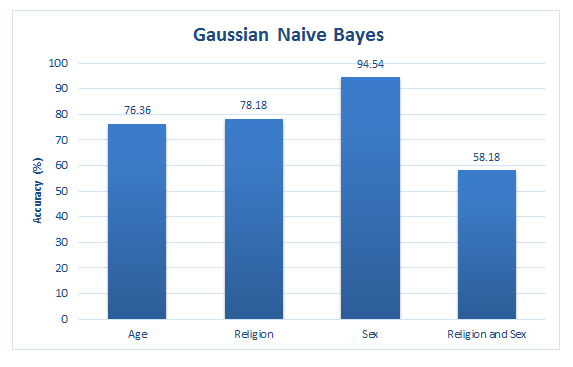
\includegraphics[scale=0.8]{./img/bayes}
				\caption{Performance diagram of Naive Bayes algorithm.} \label{fig:mapComp}
\end{figure}

\end{document}

  
